\chapter{Introduction to Neural Networks}
\begin{definition}[Artificial neuron]
	An artificial neuron (i.e. a perceptron) is a non linear parametrized function with restricted output range
\end{definition}

One example of perceptron is Rosemblatt (1958).

One problem with traditional perceptron is that it cannot solve the XOR: 
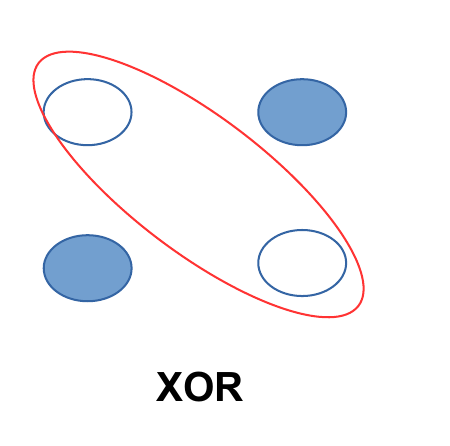
\includegraphics[scale=0.2]{xor}

because it is not linearly separable.

An idea to solve this is an {\bf MLP} (Multi Layered Perceptron), where the layers in between are intermediate results.

The problem now though is how to train an MLP. For perceptron we need to know the desired target and for hidden layers that is not the case. There are some ideas as follow. 
\newpage
{\bf Backpropagation}  was an idea to solve this problem, basically backpropagating the estimated error and updating the perceptron weights accordingly. \\
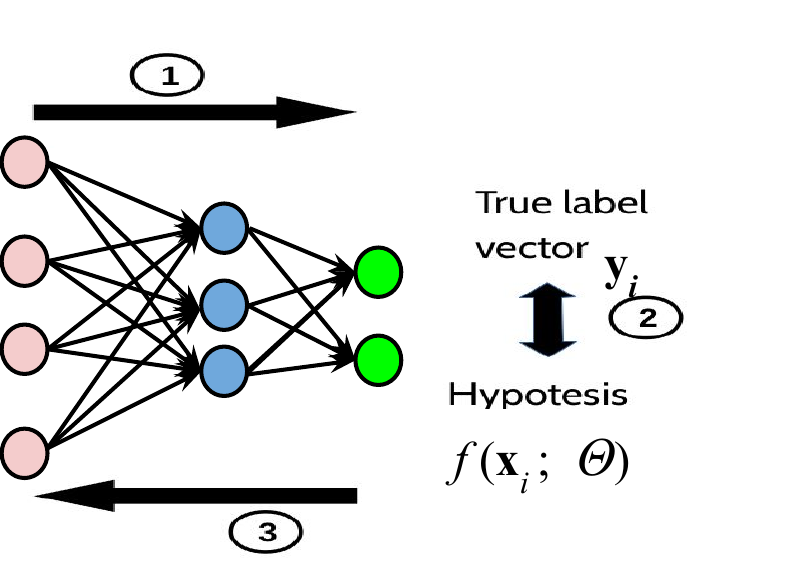
\includegraphics[scale=0.2]{backpropagation}

Now the problem was linked to the fact that neural networks cannot exploit many layers due to lack of computational power and overfitting. \\
Now neural networks reign supreme because of new findings. Raw data is always better than features and studies show that error rate is at an all time low. 

\begin{definition}[Neural Network]
	It's a composition of modules and a series of hierarchically connected functions, each with its own parameters.
\end{definition}

\section{Feedforward networks: basic elements}

The goal of a feedforward network is to approximate an idea function $f$. Information flows throughout the intermediate layers (hidden) to end on the last layer which is called output layer. \\
The function $f$ is a composite of the functions that comprise all the layers.\\
The {\bf training} is no different from other ML algorithms. \\
There are several modeling choices to be made:\\
{\bf COST FUNCTION}: for example cross-entropy or square loss\\
{\bf OUTPUT UNITS}: it's preferable to output probabilities (softmax) rather than linear outputs which could generate difficult gradient descent attributes. \\
The hidden unit accepts the input x and produces the output $h(z)$. The choice of $h$ (called {\bf ACTIVATION FUNCTION}) varies greatly. \\
{\bf ARCHITECTURE}\\
{\bf OPTIMIZATION }(see later)
\section{Backpropagation}
There are three steps to this:
\begin{enumerate}
	\item Feedforward propagation
	\item Use the computed output to calculate a scalar cost depending on the loss function
	\item Backpropagation
\end{enumerate}

The main idea of backpropagation is to use gradient descent. We do not know how or which of the hidden units are wrong but we can infer with gradient descent the speed at which we're getting farther from the correct output.

